\chapter{\label{chap:entwurf}Konzeption}
Die erarbeiteten Anforderungen an ein Ampelinformationssystem für FahrradfahrerInnen werden in diesem Kapitel für die Konzeption angewendet. Beginnend mit dem Aufbau der Anwendung werden in den folgenden Abschnitten das Design, die von der Anwendung genutzten Daten, Anwendungsfälle, die Architektur und schließlich die Komponenten der Entwicklumgsumgebung, welche eingesetzt werden aufgeführt. 
\section{Anwendungsaufbau}
Die Anwendungsarchitektur verwendet die Vorgaben für Android-Applikationen. So wird die Hauptkomponente mit Hilfe sogenannter \glspl{Activity} realisiert. Als Basisklasse definiert eine \gls{Activity} das \gls{UI} einer mobilen Anwendung, stellt also die Ansicht mit der BenutzerInnen interagieren können bereit.\\
Eine \gls{Activity} wird von der Bibliotheksklasse \texttt{android.app.Activity} abgeleitet, als Klasse implementiert und muss ind er Manifestdatei der \gls{App} aufgeführt werden. \cite{android_activity} \\
In der zu entwickelnden Fahrradapplikation wird keine Navigation innerhalb der Anwendung vonnöten sein, weshalb nur eine \gls{Activity} implementiert wird.
% DATENGRUNDLAGE
\section{Datengrundlage}
\subsection{Ampeldaten}
Von der Verkehrsleitzentrale zur Verfügung gestellt.\\
Strecke: Bornholmer Straße/Björnsonstraße bis zur Ecke Prenzlauer Allee/Ostseestraße und zurück. 
Eine verkehrsabhängige \gls{LSA} ist dabei, diese wird nicht beachtet, da Genauigkeit nicht hoch genug sein kann.
Position und Signalpläne\\
Sind ggf. umzuwandeln, bzw anzupassen + manuell zu übernehmen da Format = .pdf.\\
\subsection{Positionsdaten + Geschwindigkeit}
% ### USE CASES ###
\section{Anwendungsfälle}
Aus den in Kapitel \ref{chap:anforderungen} beschriebenen Anforderungen und den in Kapitel \ref{chap:szenarien} erarbeiteten Szenarien ergeben sich die folgenden fünf Use-Cases, die von der Anwendung erfüllt werden sollen.\\
\begin{table}[H]
\centering
	\begin{tabular}{@{}>{\columncolor[HTML]{ECF4FF}}l ll@{} p{0.1\textwidth}p{0.4\textwidth}p{0.4\textwidth}} \toprule	
\multicolumn{1}{c}{\cellcolor[HTML]{ECF4FF}\textbf{ID}} & \multicolumn{1}{c}{\cellcolor[HTML]{ECF4FF}\textbf{Anwendungsfall}} & \multicolumn{1}{c}{\cellcolor[HTML]{ECF4FF}\textbf{Beschreibung}} \\ \hline
% UC1
\multicolumn{1}{l}{\cellcolor[HTML]{ECF4FF}\textbf{UC2}} & \multicolumn{1}{p{0.35\textwidth}}{Ich fahre langsamer, um die grüne Ampel zu passieren}
& \multicolumn{1}{p{0.55\textwidth}}{Der Countdown der aktuellen Ampelphasendauer wird sekündlich aktualisiert und zusätzlich zur Aufforderung langsamer zu fahren angezeigt} \\ \midrule
% UC2
\multicolumn{1}{l}{\cellcolor[HTML]{ECF4FF}\textbf{UC1}} & \multicolumn{1}{p{0.35\textwidth}}{Ich fahre schneller, um die grüne Ampel zu passieren}
& \multicolumn{1}{p{0.55\textwidth}}{Es wird eine Beschleunigungsaufforderung ausgesprochen. Unterstützend wird der Countdown der aktuellen Ampelphasendauer sekündlich aktualisiert und zusätzlich angezeigt} \\ \midrule
% UC3
\multicolumn{1}{l}{\cellcolor[HTML]{ECF4FF}\textbf{UC3}} & \multicolumn{1}{p{0.35\textwidth}}{Ich halte meine Geschwindigkeit, um die grüne Ampel zu passieren}
& \multicolumn{1}{p{0.55\textwidth}}{Die aktuelle Geschwindigkeit ist genauso hoch wie die berechnete Empfehlungsgeschwindigkeit. Es wird angezeigt, dass kein Handlungsbedarf besteht, also das Tempo gehalten werden kann.}\\ \midrule
% UC4
\multicolumn{1}{l}{\cellcolor[HTML]{ECF4FF}\textbf{UC4}} & \multicolumn{1}{p{0.35\textwidth}}{Ich muss in jedem Fall bei roter Ampel anhalten}
& \multicolumn{1}{p{0.55\textwidth}}{Die berechnete Empfehlungsgeschwindigkeit übersteigt die festgelegte Höchstgeschwindigkeit oder die zu erreichende Beschleunigung ist in dem Maße nicht zu erreichen, also ist die Distanz zur Ampel zu lang. Eine Anzeige mit dem Signal "'keine Weiterfahrt ist möglich"' erscheint.}\\ \midrule
%UC5
\multicolumn{1}{l}{\cellcolor[HTML]{ECF4FF}\textbf{UC5}} & \multicolumn{1}{p{0.35\textwidth}}{Es ist nicht möglich eine Vorhersage zu treffen}
& \multicolumn{1}{p{0.55\textwidth}}{Eine verkehsrabhängige Ampel mit individueller Steuerung nähert sich. Es ist dem System nicht möglich eine wahrscheinliche Vorhersage zu treffen und so die entsprechende Empfehlung auszusprechen. Es wird \textit{ein gelbes Fragezeichen, symbolisch dafür} angezeigt.}\\ \bottomrule
\end{tabular}
	\caption{Anwendungsfälle}
	\label{tab:uc}
\end{table}
Das in Abbildung \ref{fig:uc} gezeigte Use-Case-Diagramm veranschaulicht die in der obigen Tabelle \ref{tab:uc} aufgeführten Anwendungsfälle.  
\begin{figure}[H]  
    \centering  
    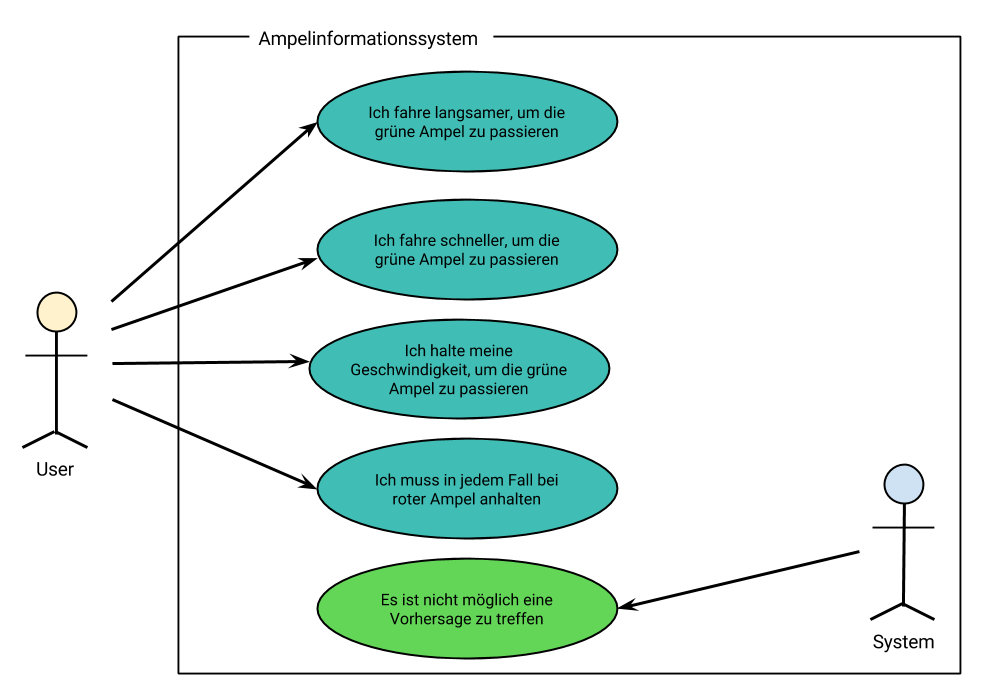
\includegraphics[width=\textwidth]{uc} 
    \rule{35em}{0.5pt}
    \caption{Use-Case-Diagramm}
    \label{fig:uc}
\end{figure}
\section{Klassenarchitektur}
Die einzelnen Klassen der Anwendung werden ihrer Aufgaben entsprechend in Pakete gegliedert?\\
Die zu erstellende Anwendung erhält den Namen AIS, das Hauptpaket den Namen \texttt{de.jacoba.ais}. AIS steht für Ampel-Informationssystem und ist der vorläufige Name der Anwendung. \\\\
In dem Paket befindet sich die \texttt{MainActivity}, die Hauptklasse der Android-Applikation. Sie definiert die grafische Oberfläche der Anwendung und stellt die notwendigen Methoden bereit. \\
\texttt{GPSTracker} trackt kontinuierlich die Position des Endgeräts.\\
\texttt{SpeedAdvisory} enthält Berechnungsmethoden zur Ermittlung der optimalen Geschwindigkeit.\\
 \texttt{util} = Hilfsklassen -->
% ### Design ###
\section{Das Design}
Aus den Anforderungen an die graphische Oberfläche in Kapitel \ref{chap:anforderungen} entsteht das Design. Durch die überschaubare Anzahl an Funktionalitäten kann der Aufbau einfach gehalten werden. Aus den Empfehlungsanzeigen, welche den Systemzuständen entsprechen sind vier Fenster abzuleiten. Die folgende Abbildung zeigt den Entwurf der Benutzeroberfläche.
Abbildung \ref{fig:stop} zeigt die grapfische Umsetzung des Zustands \textit{a}, in dem die Ampelschaltung keine Weiterfahrt ermöglicht. Es wird ein großer roter Kreis mit einem schwarzen Kreuz verwendet. Rot ist eine Signalfarbe und steht auch bei Ampeln für "'Halt"' oder "'Stop"'. Auch das Kreuz wird häufig als \textit{verweigerndes} Symbol eingesetzt und ist somit intuitiv als solches erkennbar.\\
Abbildung \ref{fig:yeah} setzt die Visualisierung des Zustands \textit{b} um, bei dem man mit der aktuellen Geschwindigkeit in der Grünen Welle mitschwimmt, um. Hier wird ist ein großer grüner Kreis verwendet, in der Mitte steht "'ok"'. Durch die nicht alleinige Benutzung der Ampelfarben Rot und Grün ist die Ansicht auch für Menschen mit einer Rot-Grün-Sehschwäche eindeutig interpretierbar.
\begin{figure}[H]
        \centering
           \begin{subfigure}[t]{0.18\textwidth}
                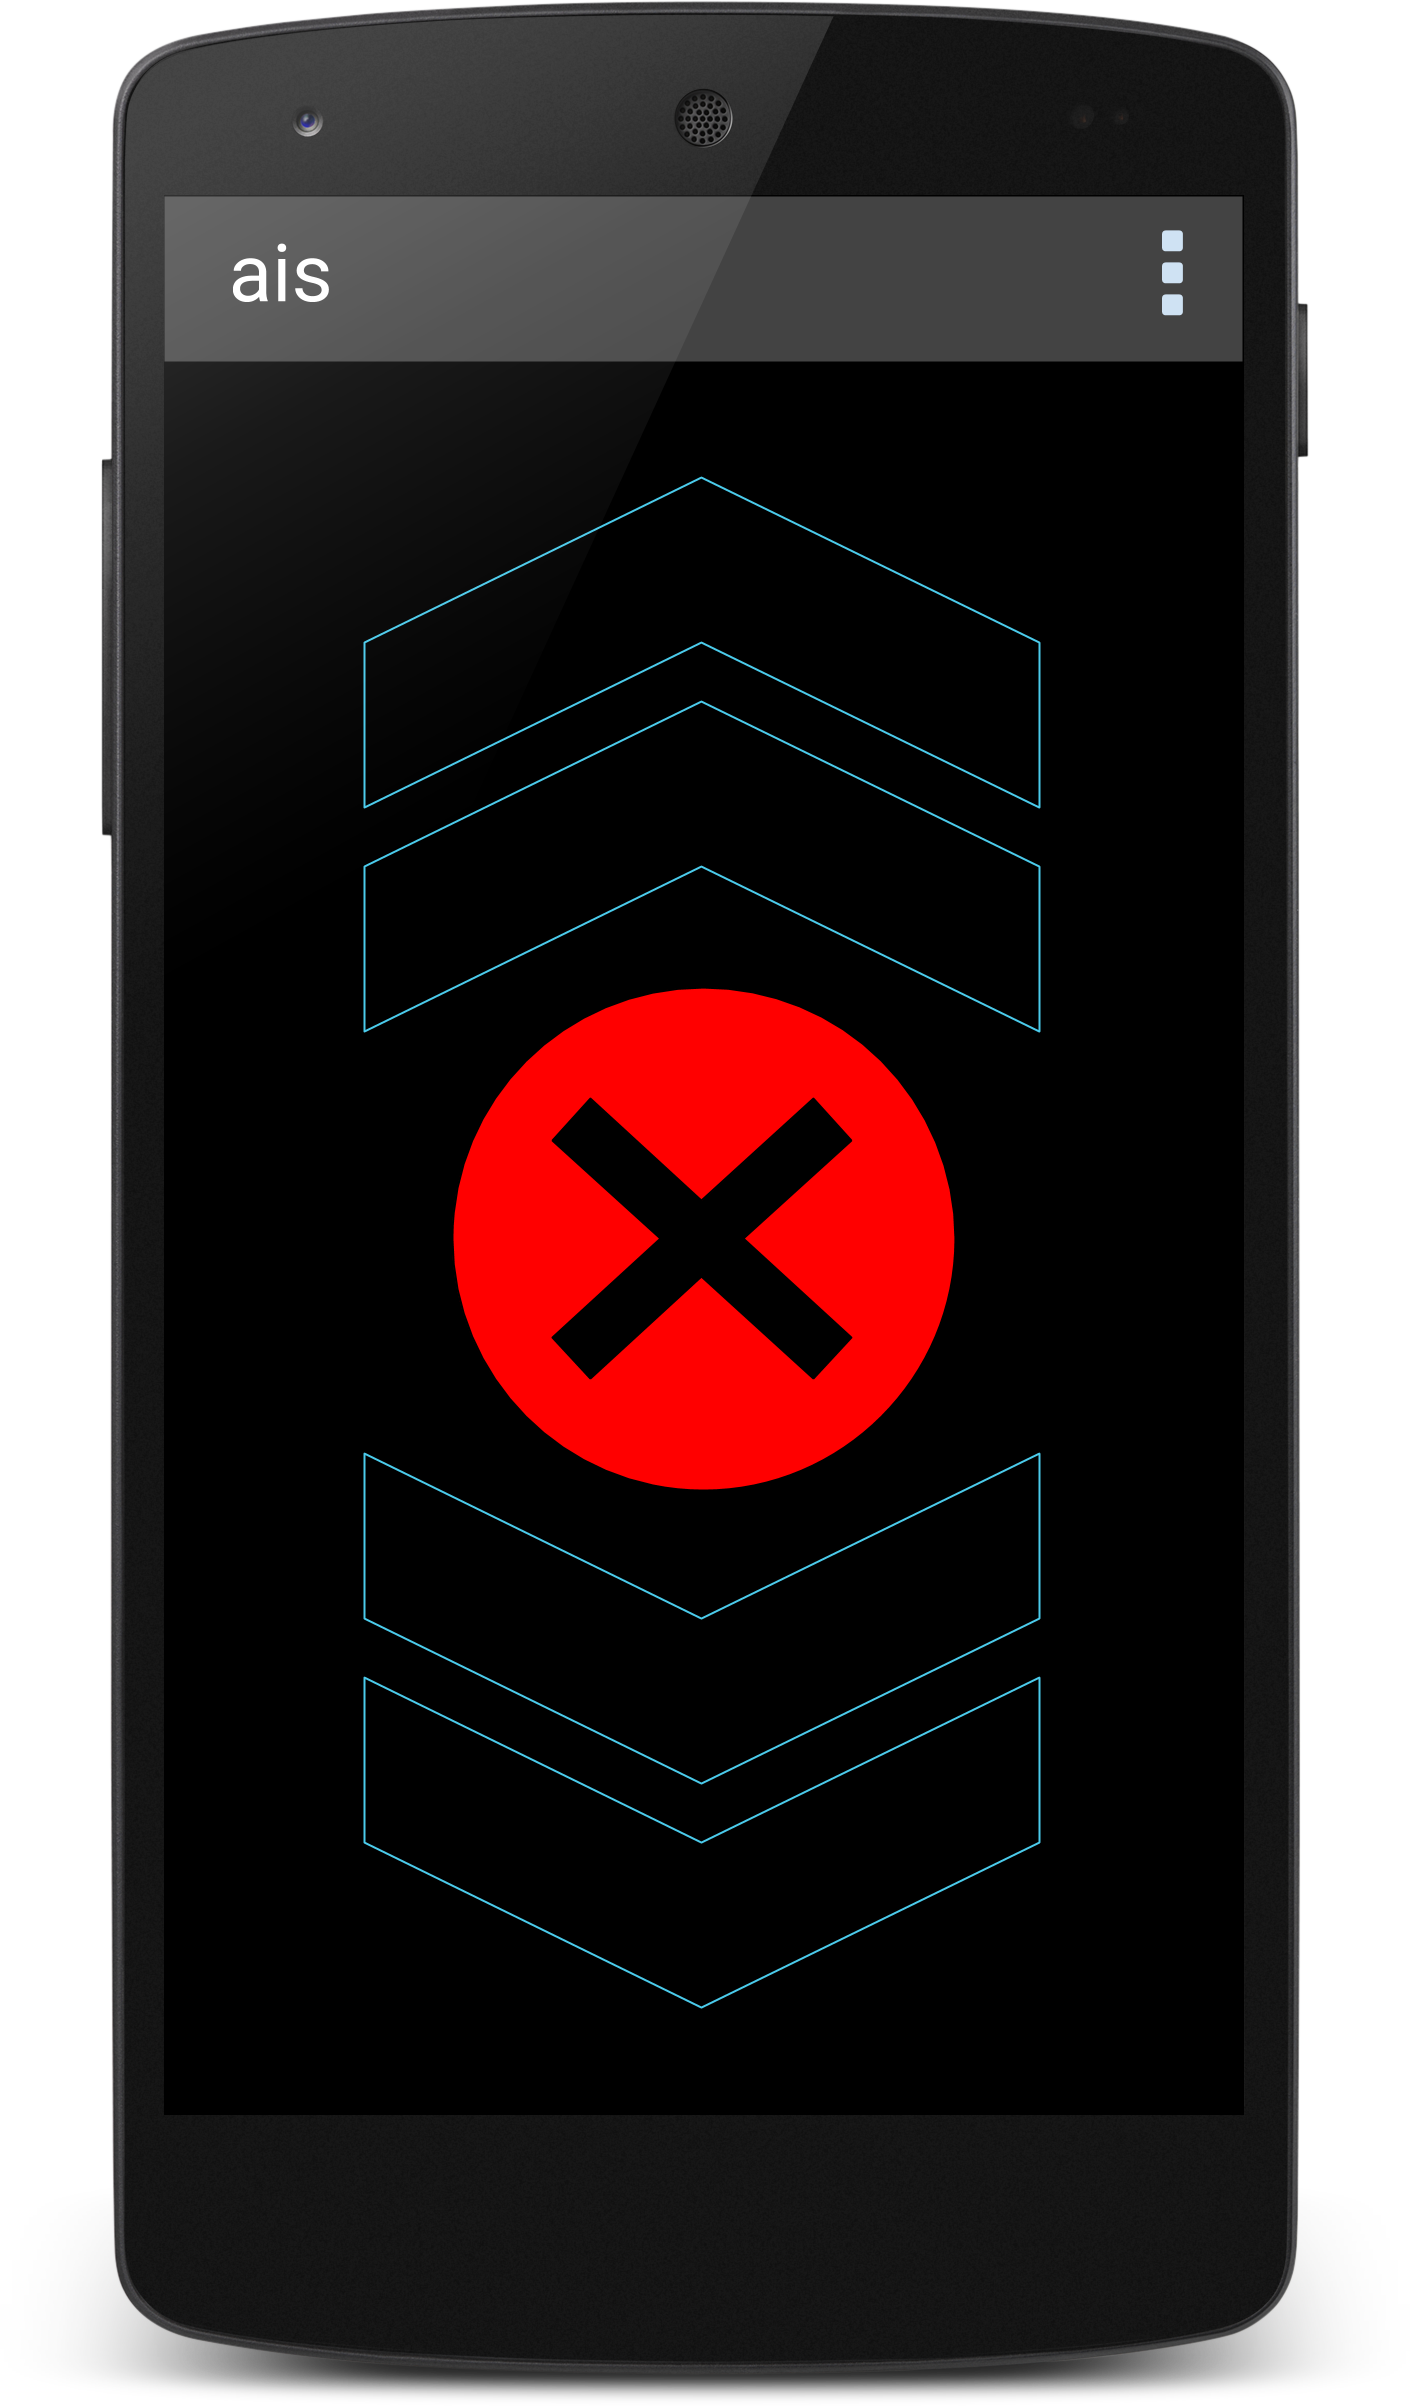
\includegraphics[width=\textwidth]{stop}
                \caption[Systemzustand a]{Anhalten an roter Ampel in jedem Fall erforderlich}
                \label{fig:stop}
        \end{subfigure}
           ~ 
              \begin{subfigure}[t]{0.18\textwidth}
                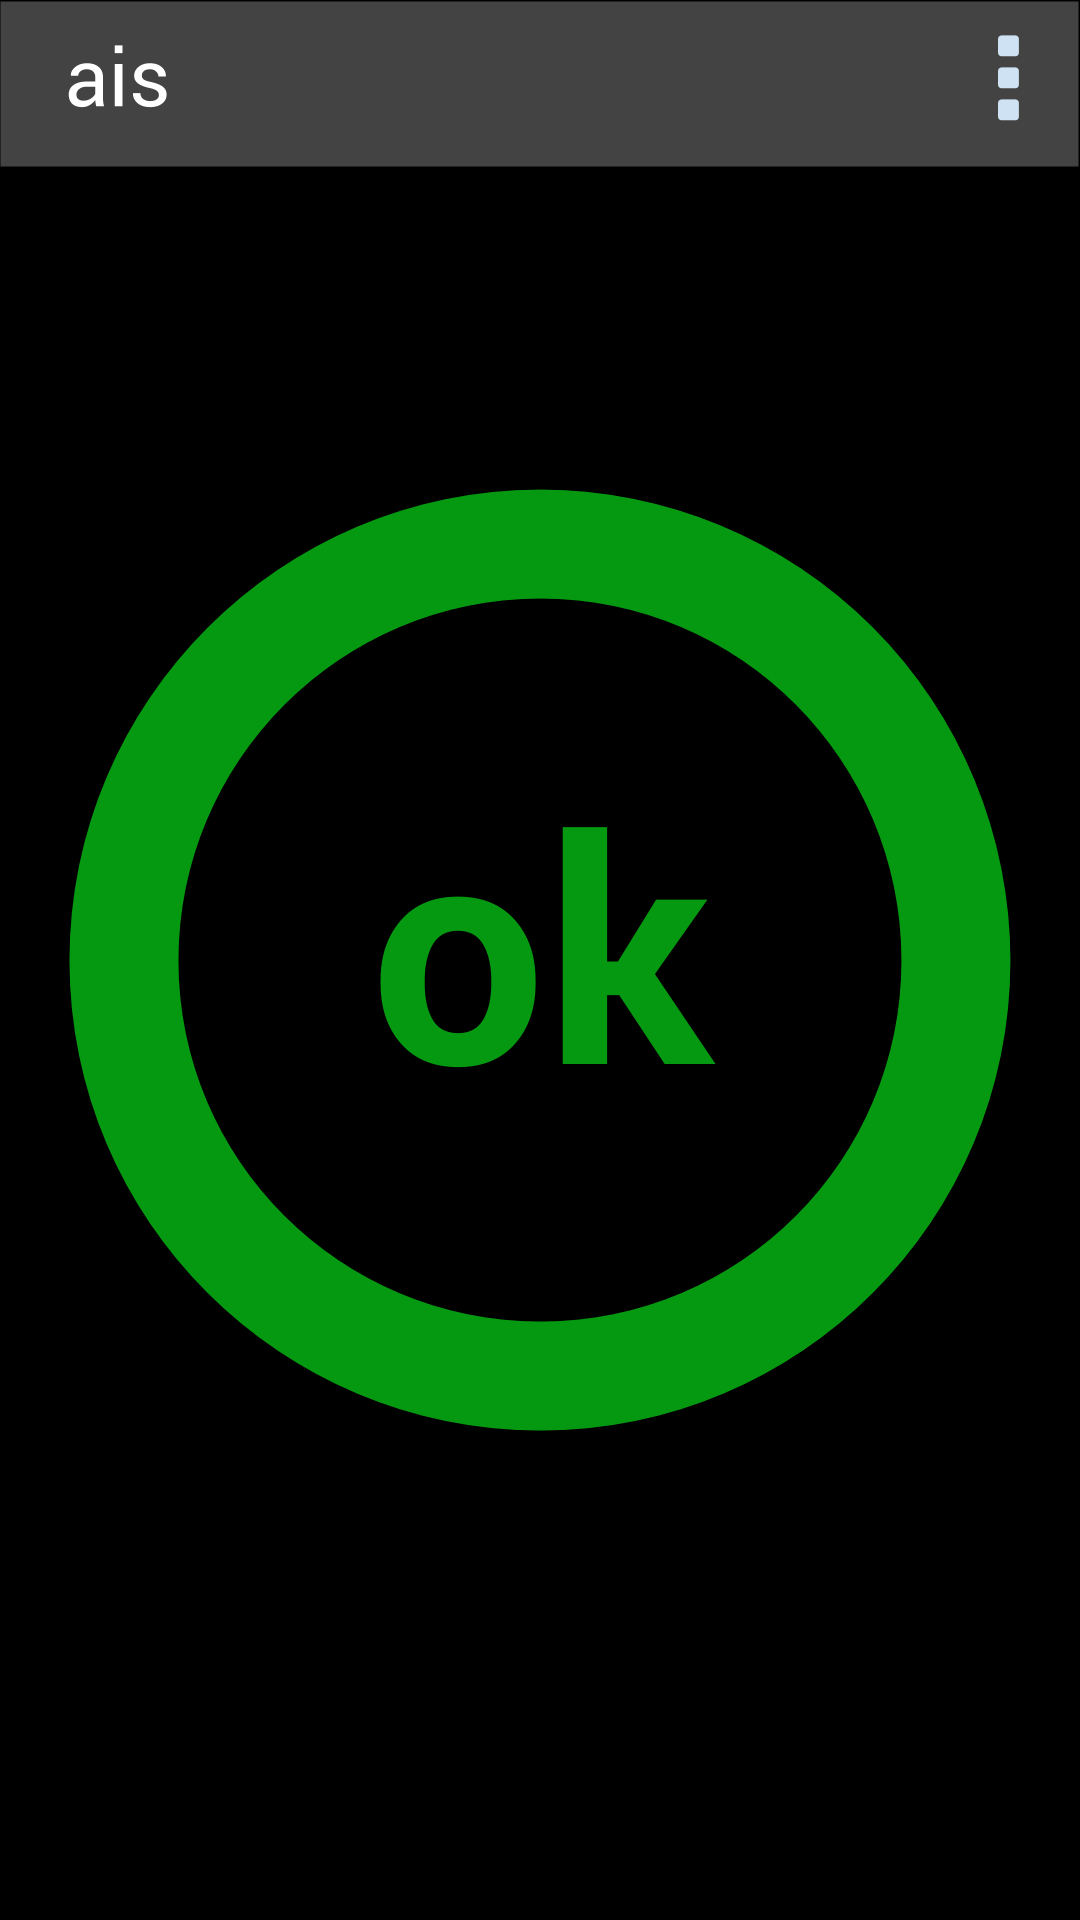
\includegraphics[width=\textwidth]{yeah}
                \caption[Systemzustand b]{Kein Aktionsbedarf}
                \label{fig:yeah}
        \end{subfigure}
           ~
        \begin{subfigure}[t]{0.18\textwidth}
                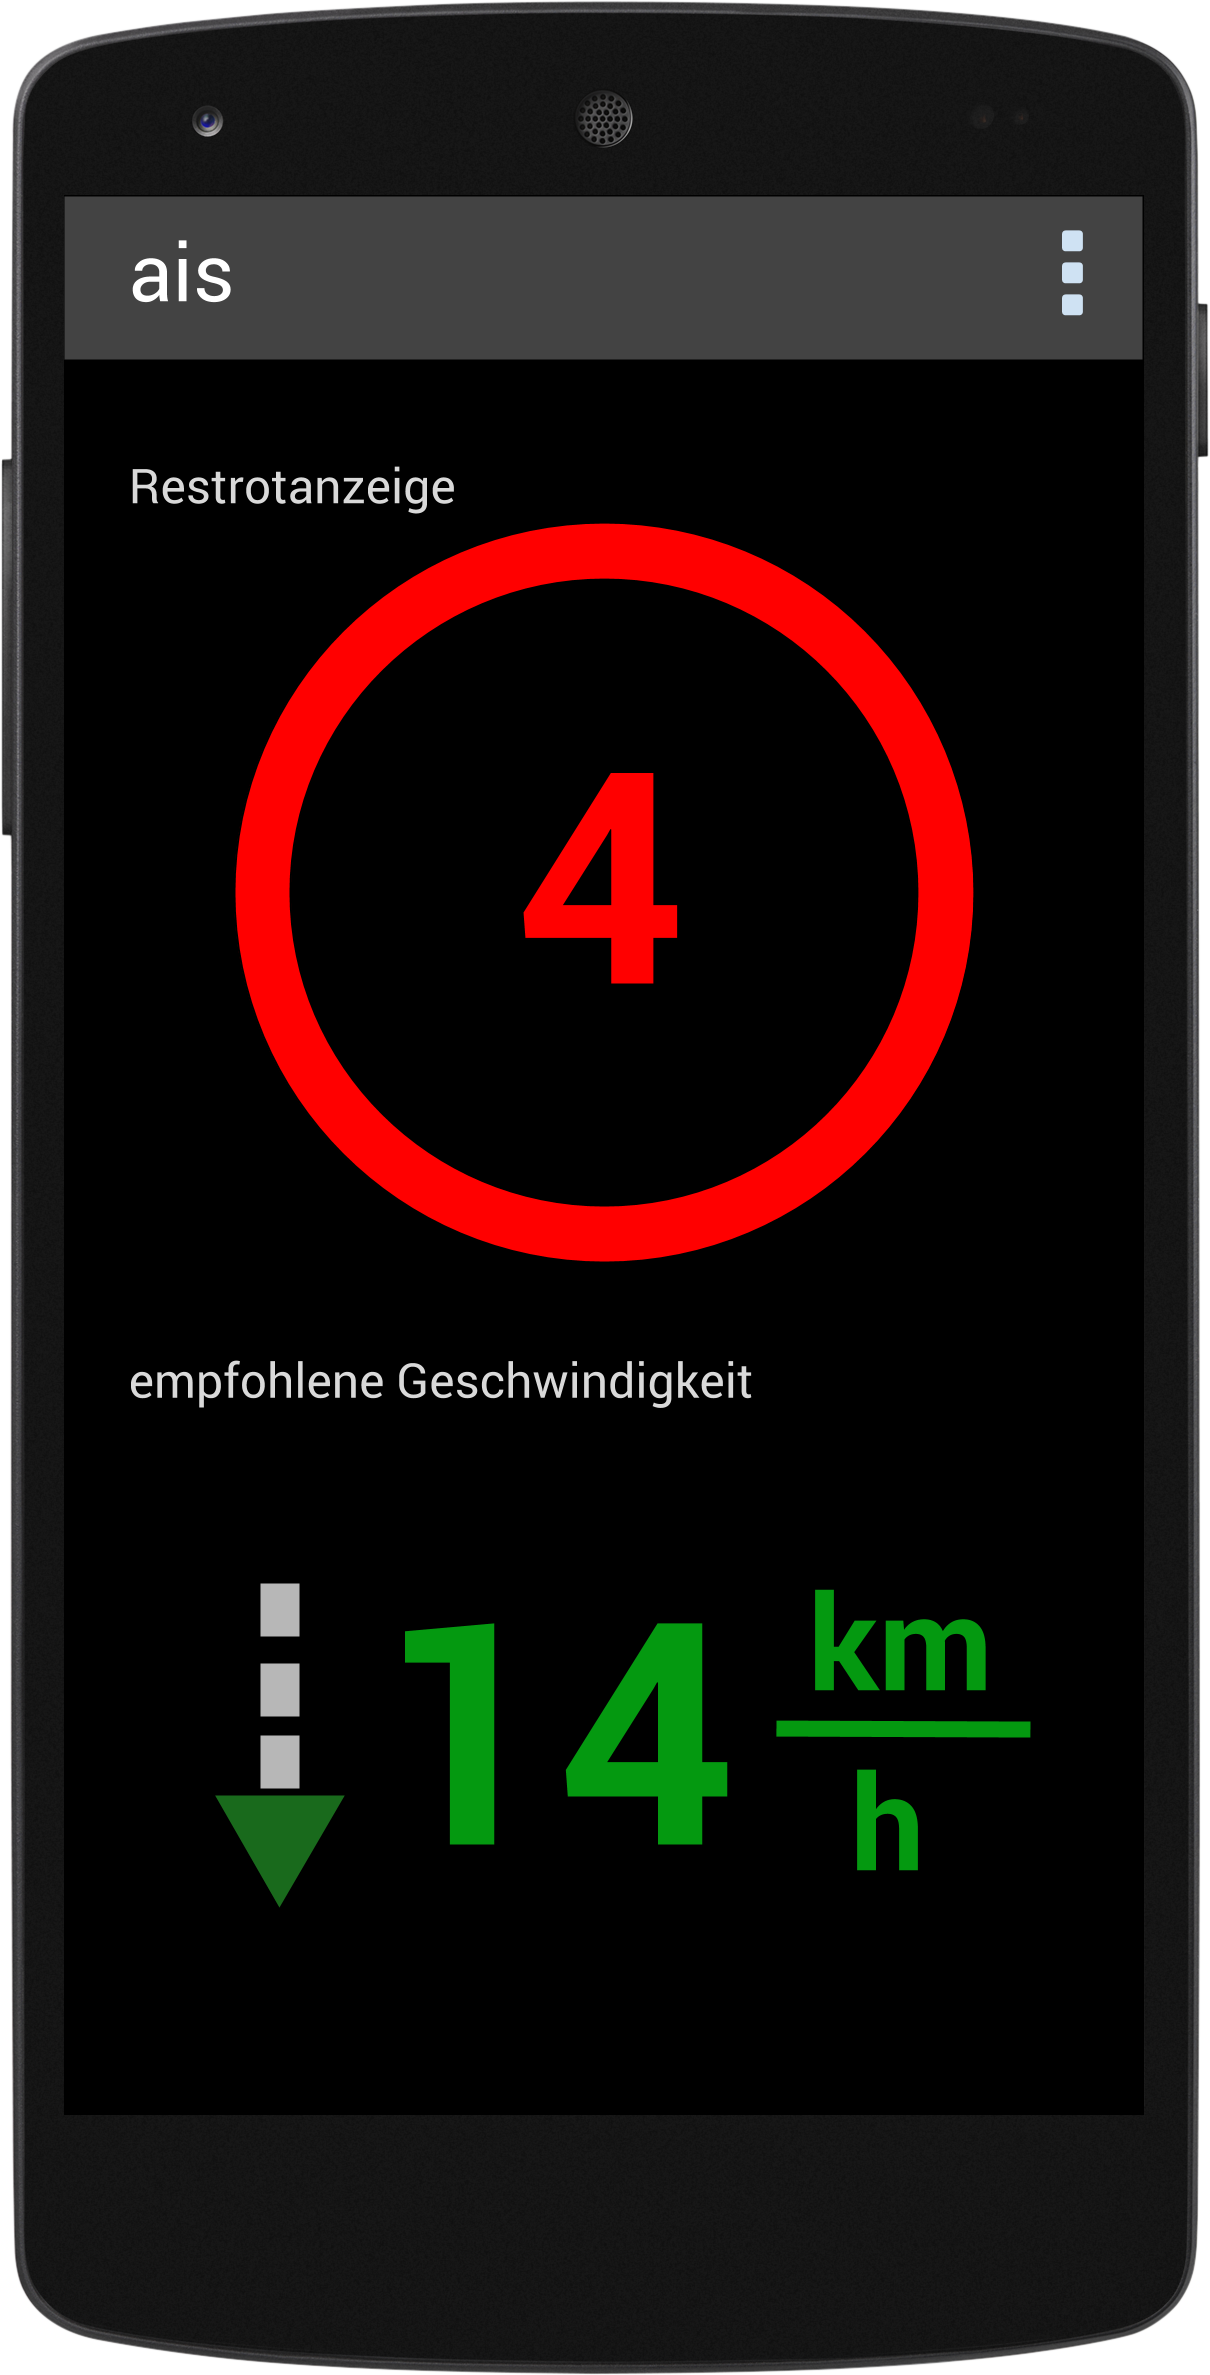
\includegraphics[width=\textwidth]{langsamer}
                \caption[Systemzustand c]{Weiterfahrt durch Verlangsamung  möglich}
                \label{fig:langsamer}
        \end{subfigure}
        ~
        \begin{subfigure}[t]{0.18\textwidth}
                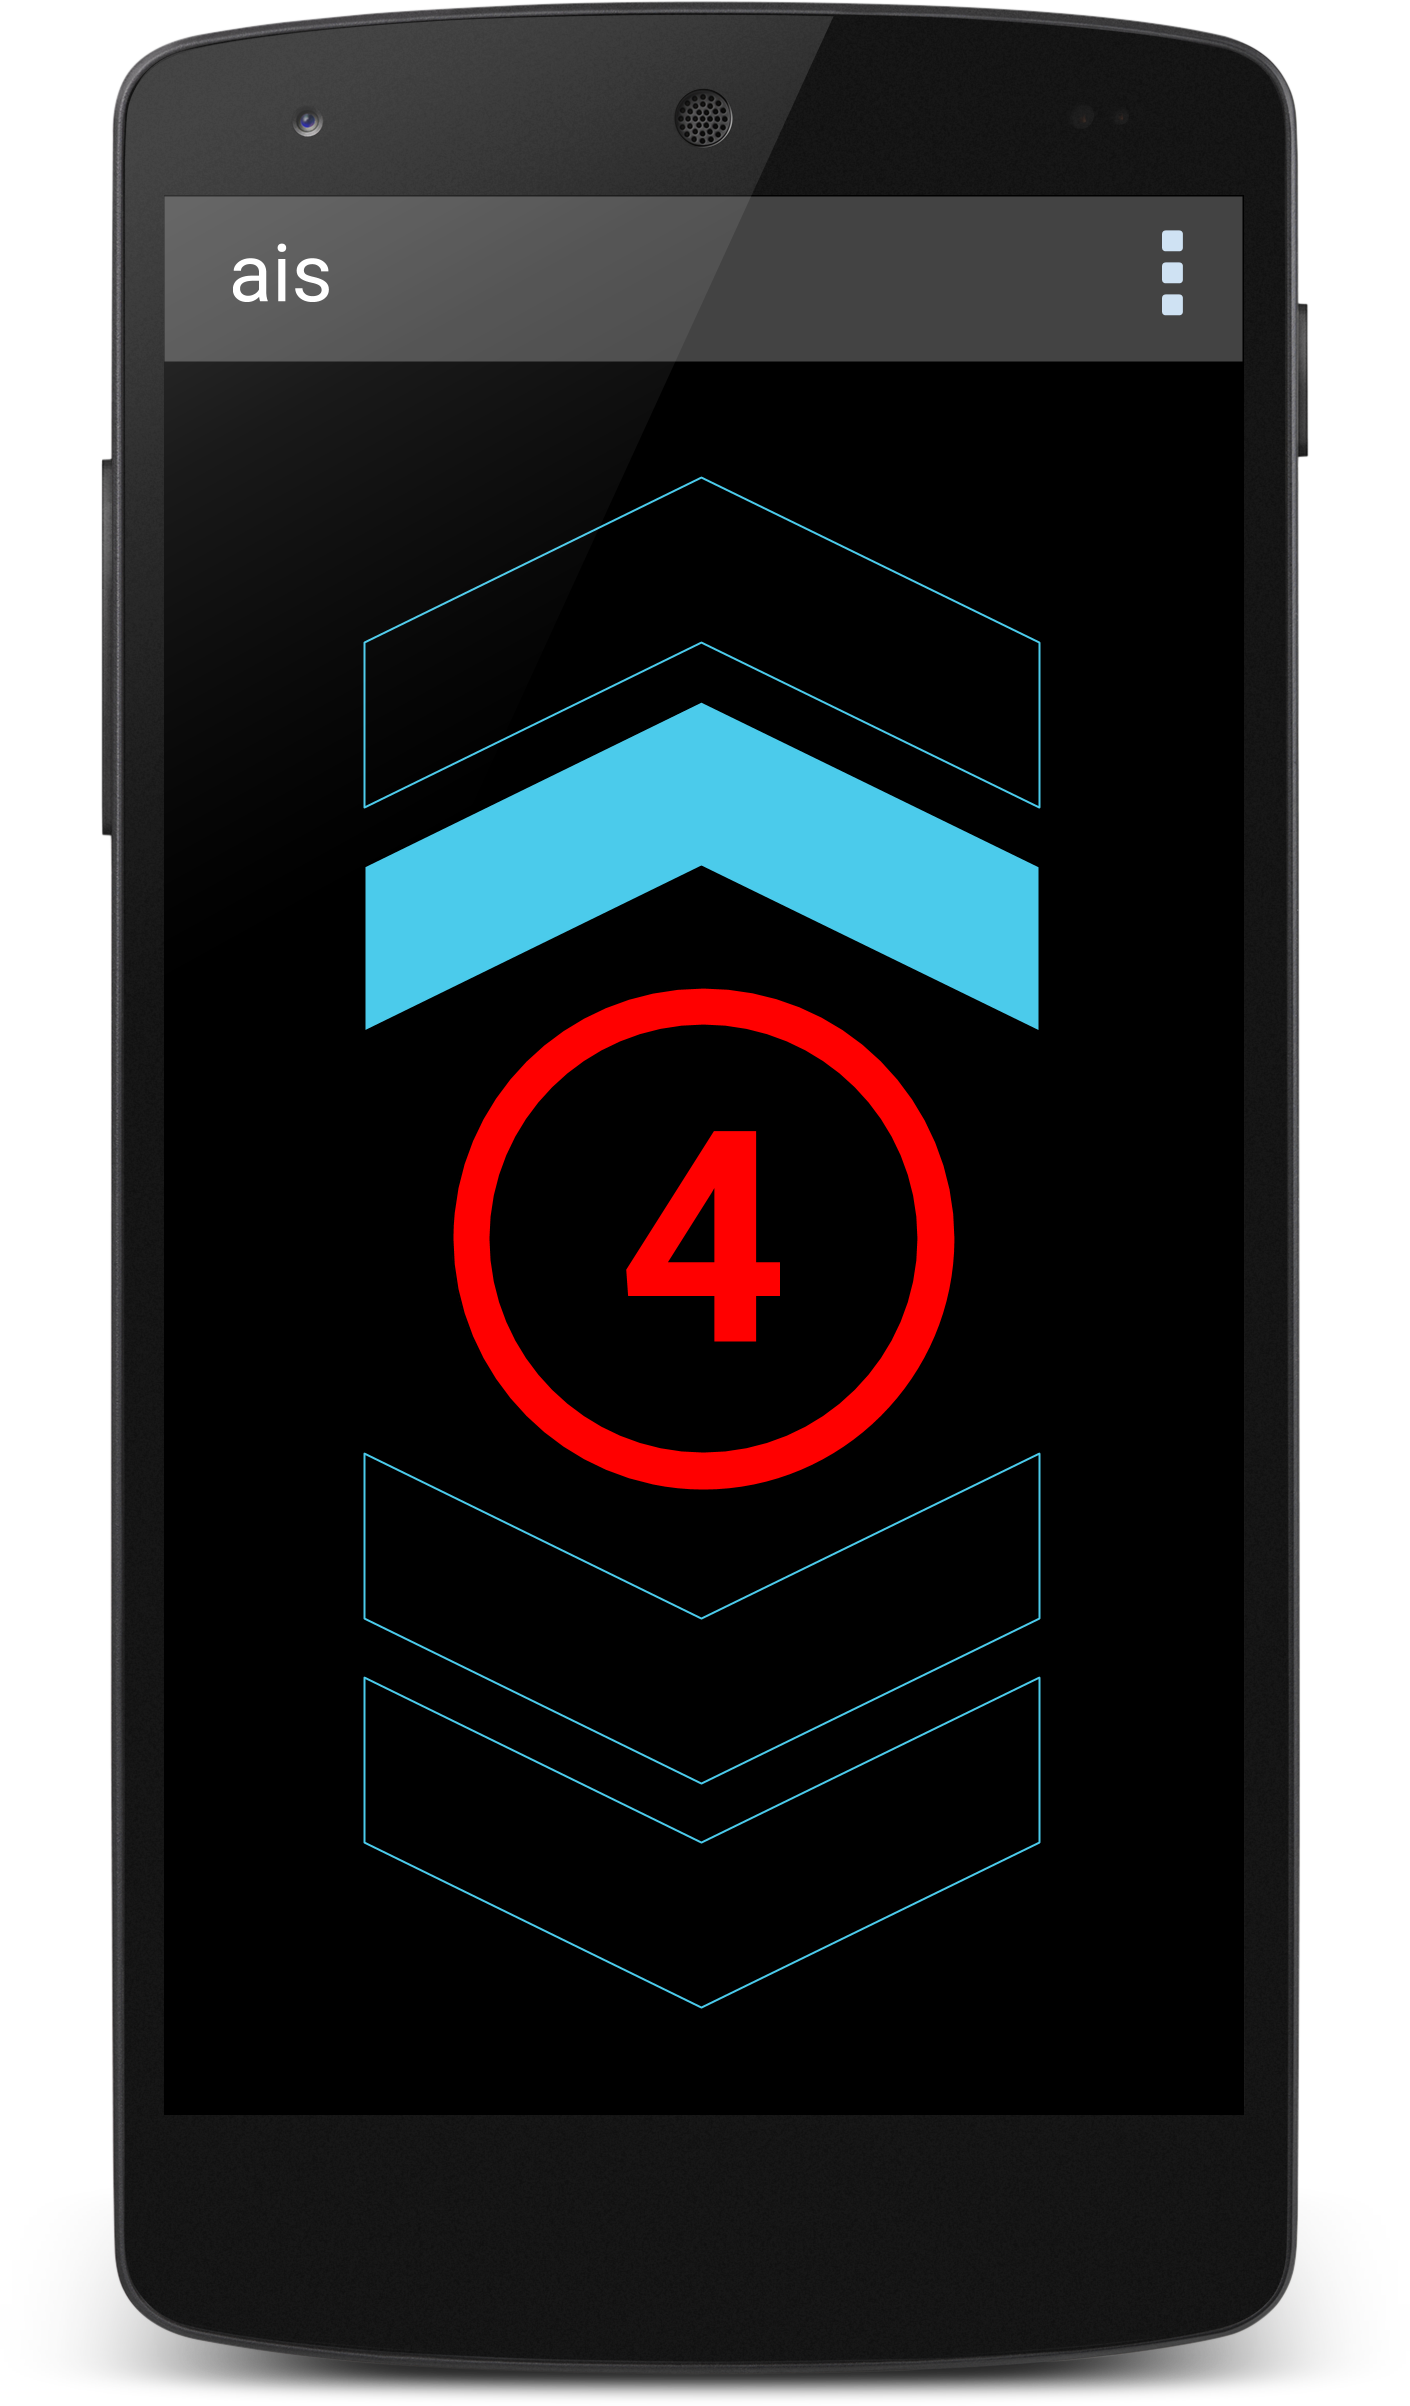
\includegraphics[width=\textwidth]{schneller}
                \caption[Systemzustand d]{Weiterfahrt durch Beschleunigung möglich}
                \label{fig:schneller}
        \end{subfigure} 
        ~ 
        \begin{subfigure}[t]{0.18\textwidth}
        	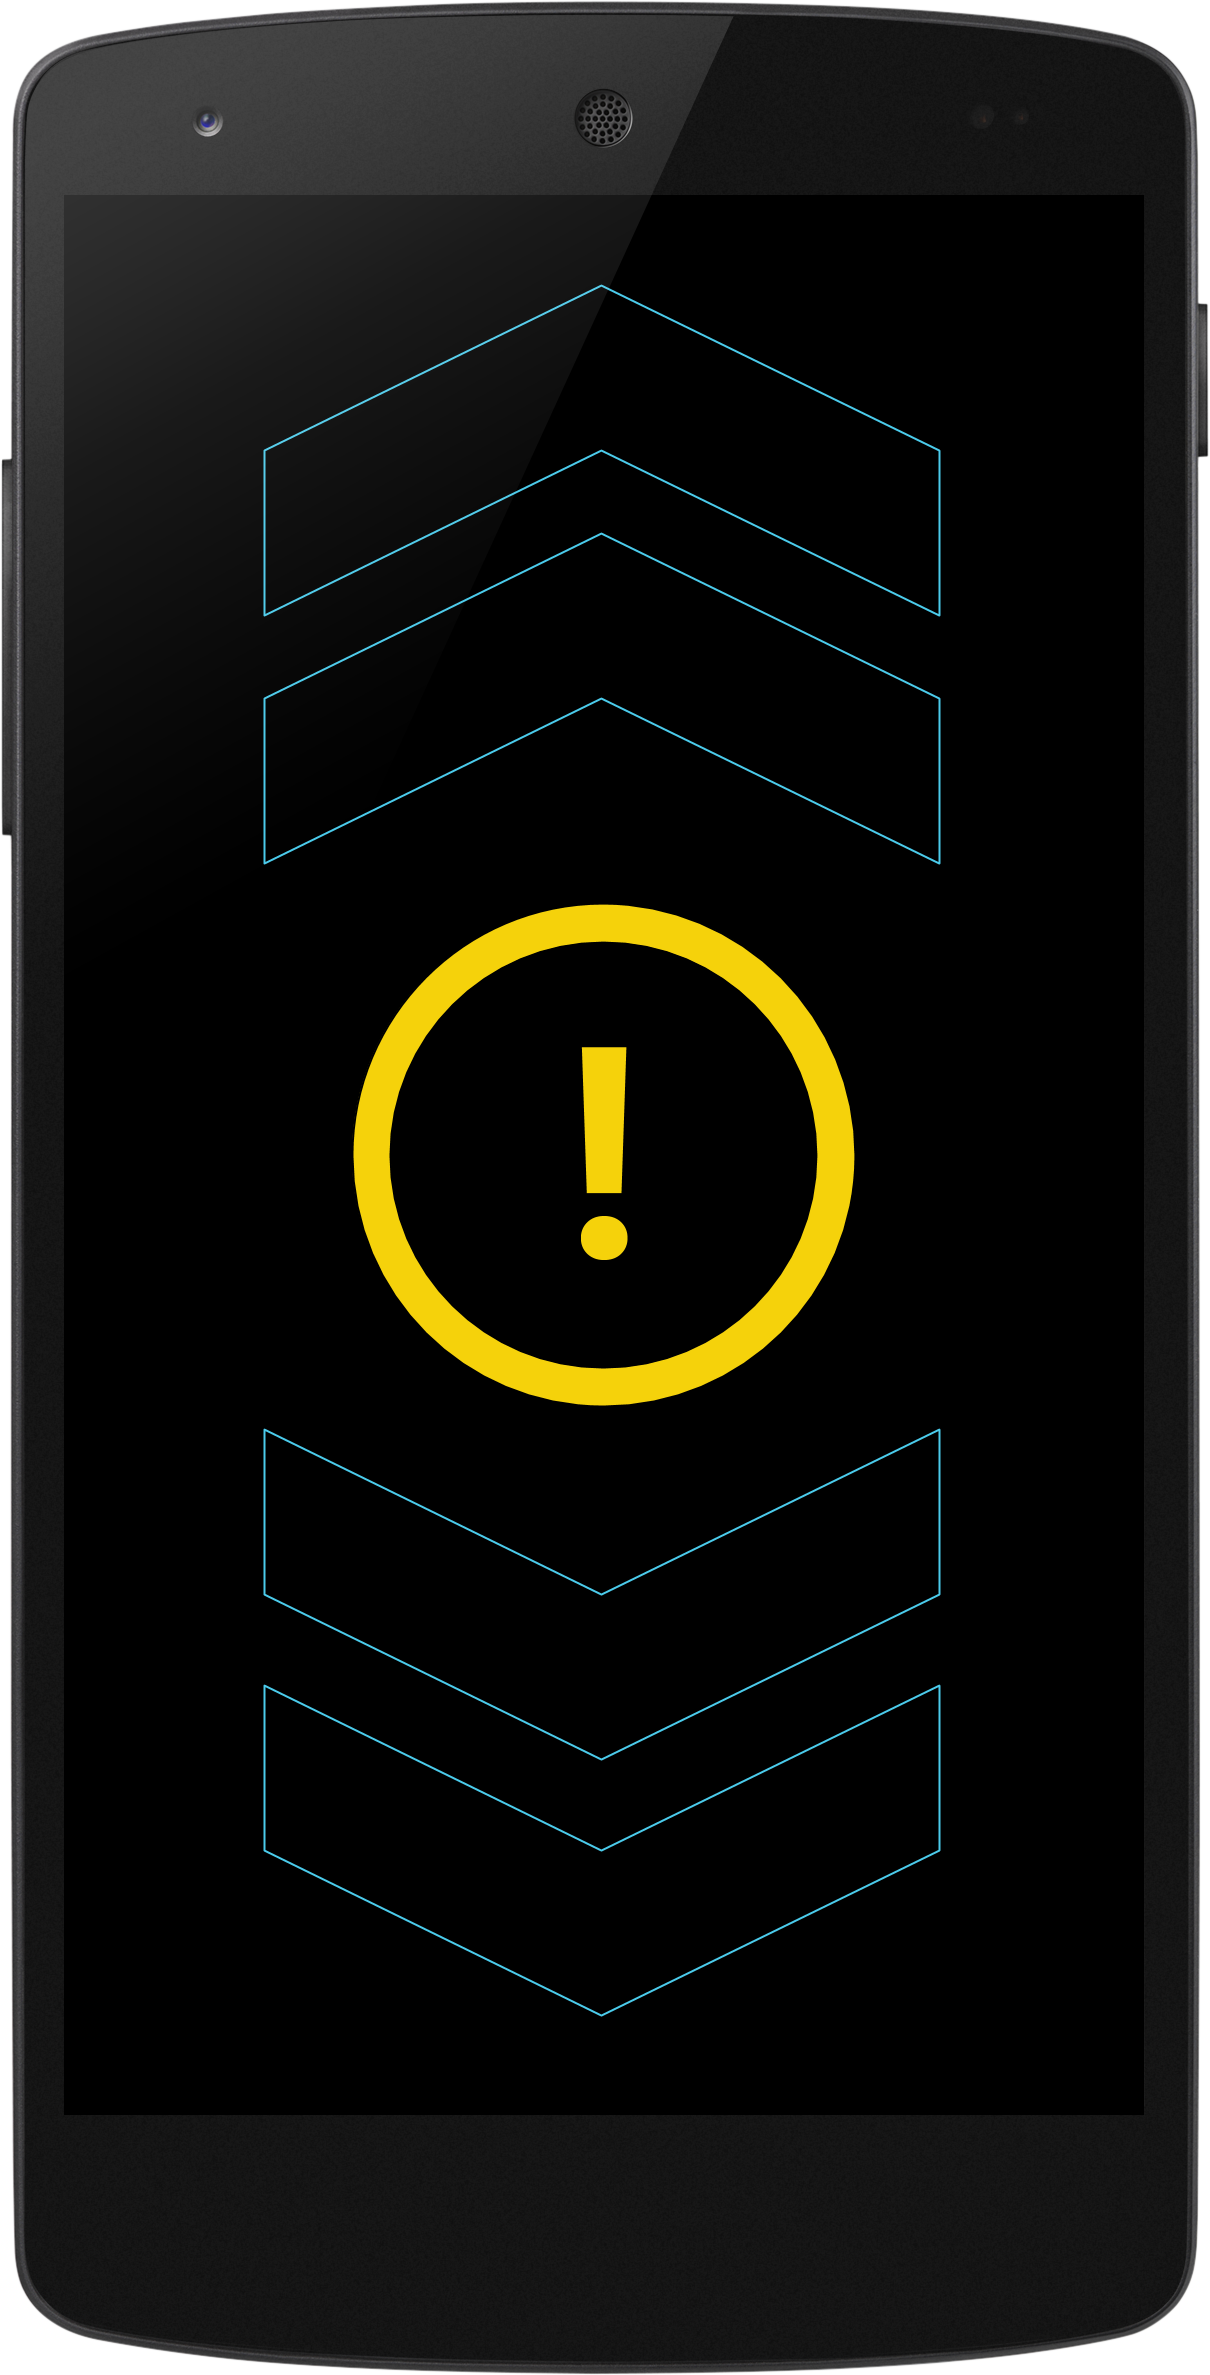
\includegraphics[width=\textwidth]{mep}
        	\caption[Systemzustand e]{Keine Vorhersage möglich}
            \label{fig:meh}
        \end{subfigure} 
        \rule{35em}{0.5pt}   
        \caption[Systemzustände im Ampelbereich]{Entwurf des Designs anhand der Systemzustände}
        \label{fig:mockup}
\end{figure}
Die Abbildungen \ref{fig:langsamer} und \ref{fig:schneller} für die Zustände \textit{c} und \textit{d} sind in der Anordnung der Elemente identisch. Mittig im Bild ist eine eingekreiste rote Zahl die den Countdown der Restrotanzeige darstellt. Sie wird also mit jeder Sekunde aktualisiert. Ober- und unterhalb des Countdowns befinden sich jeweils zwei hellblaue Pfeile. Je nach Differenz der aktuellen zur berechneten Geschwindigkeit sind ein oder zwei Pfeile ausgefüllt. Wird also empfohlen viel schneller zu fahren, sind die oberen Pfeile aktiv, bei der Aufforderung etwas das Tempo zu drosseln der untere. Es sind immer alle Pfeile zu sehen. Durch die Anzeige "'ein von zwei"' ist die Bedeutung der Geschwindigkeitsstufen klarer. Als Farbe für die Pfeile wurde Hellblau gewählt. Sie unterscheidet sich sowohl farblich als auch in der Helligkeitsstufe zu den anderen Farben und steht im hohen Kontrast zu dem Hintergrund. Auf schwarzem Hintergrund wirken die Farben intensiver und sind so auch aus dem Augenwinkel leichter zu erkennen und unterscheiden. Die in Abbildung \ref{fig:meh} gezeigte Darstellung erscheint, wenn keine Vorhersage möglich ist weil die Ampel verkehrsabhängig und die Vorhersage dadurch zu ungenau wird. Als Farbe wurde die dritte Ampelfarbe Gelb gewählt, was ja weder Rot für Anhalten, noch grün für Weiterfahren ist und so signalisiert, die Anwendung kann keine Empfehlung aussprechen. Das mittig platzierte Fragezeichen unterstützt die Aussage.\\
Die aktuelle Geschwindigkeit wird bewusst nicht angezeigt. Auch nicht die Progressionsgeschwindigkeit. Die Differenz ist beim Fahrrad nicht so hoch wie bspw. im Auto. Bei einer Varianz von wenigen km/h genügt die Anzeigevariante "'schneller"' und "'noch schneller"'.
\section{Theorie ?}
\section{Entwicklungsumgebung ?}
Für die Erstellung wird Folgendes verwendet:
\begin{itemize}
	\item Android Studio
	\item ADT Bundle..., SDK, 
	\item SQLite
	\item Diagramme und Abbildungen
\end{itemize}
